\documentclass{beamer}
\usepackage{framed}
\usepackage{graphicx}

\begin{document}
	\section{Integer Programming - Lecture 8B}
\subsection{Binary Integer Problems}

\begin{frame}
\frametitle{Zero-One Integer Problems}
\begin{itemize}
\item Zero-one linear programming involves problems in which the variables are restricted to be either 0 or 1. 
\item Note that any bounded integer variable can be expressed as a combination of binary variables.
\end{itemize}

\end{frame}
%======================================= %

\subsection{Capital Budgeting}
\begin{frame}
\frametitle{Capital Budgeting}
\Large
\begin{itemize}
\item	A firm has $n$ projects that it would like to undertake but because of budget limitations not all can be
	selected. 
\item In particular project $j$ is expected to produce a revenue of $c_j$ but requires an investment of $a_{ij}$ in the time period i for $i \in 1 \ldots m$. 
\item The capital available in time period  is $b_i$ . 
\end{itemize}
\end{frame}
%===================================== %
\begin{frame}
	\frametitle{Capital Budgeting}
	\Large
	\begin{itemize}
		\item The problem of maximising revenue subject to i
	the budget constraints can be formulated as follows: let $x_j$ = 0 or 1 correspond to not proceeding or 	respectively proceeding with project j then we have to
\end{itemize}
\begin{figure}
\centering
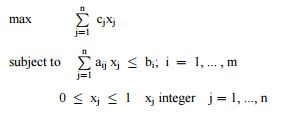
\includegraphics[width=0.9\linewidth]{capitalbudgeting}
\end{figure}

\end{frame}

\subsection{Knapsack Problems}
% - https://www.utdallas.edu/~metin/Or6302/Notes/integer.pdf
%- http://www.geeksforgeeks.org/dynamic-programming-set-10-0-1-knapsack-problem/

\begin{frame}
\begin{figure}
\centering
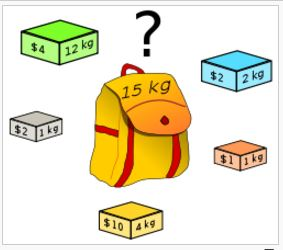
\includegraphics[width=0.9\linewidth]{knapsack}
\caption{}
\label{fig:knapsack}
\end{figure}
\end{frame}
%======================================================= %
\begin{frame}
	\frametitle{The Knapsack Problem}
\Large
\begin{itemize}
\item The knapsack problem or rucksack problem is a problem in combinatorial optimization
\item Given a set of items, each with a weight and a value, determine the number of each item to include in a collection so that the total weight is less than or equal to a given limit and the total value is as large as possible.
\end{itemize}
	
\end{frame}
%================================= %
\begin{frame}
	\frametitle{Knapsack Problems}
	\Large
	\begin{itemize}
		\item Remark: The 0-1 knapsack problems is an optimization problem.
		\item Brute force: Try all $2^n$ possible subsets (Recall definition of Power Set)
		.
		\item	Question: Any solution better than the brute-force?
	\end{itemize}
\end{frame}

\begin{frame}
	\frametitle{Knapsack Problems}
	\Large
	\begin{itemize}
	\item The most common problem being solved is the 0-1 knapsack problem, which restricts the number xi of copies of each kind of item to zero or one. 
	\item Given a set of n items numbered from 1 up to n, each with a weight wi and a value vi, along with a maximum weight capacity W,
	\end{itemize}
\begin{figure}
\centering
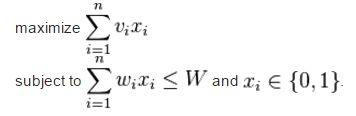
\includegraphics[width=0.7\linewidth]{01knapsack}
\caption{}
\label{fig:01knapsack}
\end{figure}
\end{frame}
\begin{frame}
	\frametitle{Knapsack Problems}
	\Large
	Here xi represents the number of instances of item i to include in the knapsack. Informally, the problem is to maximize the sum of the values of the items in the knapsack so that the sum of the weights is less than or equal to the knapsack's capacity.
\end{frame}
\begin{frame}
	\frametitle{Knapsack Problems}
\Large
The bounded knapsack problem (BKP) removes the restriction that there is only one of each item, but restricts the number $x_i$ of copies of each kind of item to an integer value $c_i$:
\begin{figure}
\centering
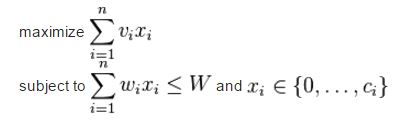
\includegraphics[width=0.7\linewidth]{boundedknapsack}

\end{figure}
\end{frame}
%================================================= %
\begin{frame}
	\frametitle{Knapsack Problems}
	\Large
The unbounded knapsack problem (UKP) places no upper bound on the number of copies of each kind of item and can be formulated as above except for that the only restriction on $x_i$ is that it is a non-negative integer.
	\begin{figure}
\centering
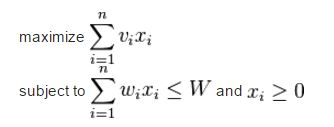
\includegraphics[width=0.9\linewidth]{unboundedknapsack}

\end{figure}

\end{frame}
%======================================================== %
\subsection{ Facility Location Problem (MILP) }
\begin{frame}
% - https://www.utdallas.edu/~metin/Or6302/Notes/integer.pdf
\end{frame}
%======================================================== %
\subsection{ Merrill Lynch Worked Example}
\begin{frame}
	Merrill Lynch is considering investments into 6 projects: A, B, C, D, E and F. Each project has an
	initial cost, an expected profit rate (one year from now) expressed as a percentage of the initial cost,

	and an associated risk of failure. These numbers are given in the table below:
\begin{figure}
\centering
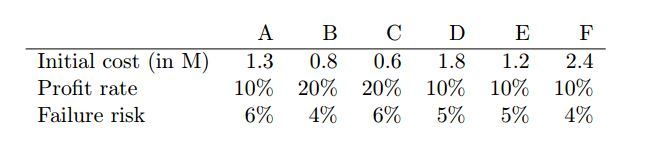
\includegraphics[width=0.9\linewidth]{MErrillLynchExample}

\end{figure}

\end{frame}

\begin{frame}
	% - https://www.utdallas.edu/~metin/Or6302/Notes/integer.pdf
\begin{itemize}
\item[a)]Provide a formulation to choose the projects that maximize total expected profit, such that Merrill
Lynch does not invest more than 4M dollars and its average failure risk is not over 5\%. \\ For example,
if Merrill Lynch invests only into A and B, it invests only 2.1M dollars and its average failure risk is
(6\%+4\%)/2=5\%.
\item[b)] Suppose that if A is chosen, B must be chosen. Modify your formulation.
\item[c)] Suppose that if C and D are chosen, E must be chosen. Modify your formulation.
\end{itemize} 
\end{frame}

\begin{frame}
	\frametitle{Branch and Bound}
\begin{framed}
The branch and bound method is a solution approach that partitions the feasible solution space into smaller subsets of solutions
\end{framed}
\end{frame}

\subsection{Depot Location Problem}
\begin{frame}
\frametitle{Depot Location Problem} %DEPOT LOCATION
\end{frame}
%====================================================== %
\subsection{Cutting Plane Algorithm}
%- CUTTING PLANE ALGORITHM FOR PURE INTEGER PROGRAMMING
%- http://www.doc.ic.ac.uk/~br/berc/integerprog.pdf
\begin{frame}
	\frametitle{Cutting Plane Algorithm} 
The rationale behind this approach is :
\begin{itemize}
\item[1.] Solve the continuous problem as an LP i.e. ignore integrality
\item[2.] If by chance the optimal basic variables are all integer then the optimum solution has been found.
Otherwise:
\item[3.] \textbf{Generate a cut} - i.e. a constraint which is satisfied by all integer solutions to the problem but not by the 
current L.P. solution.
\item[4.] Add this new constraint and go to 1 .

\end{itemize}
\end{frame}
%==================================================== %
\subsection{Fathoming}
\begin{frame}
\frametitle{Fathoming}
\Large
\begin{itemize}
\item[1] Pruning by Optimality
\item[2] Pruning by Bound
\item[3] Pruning by Infeasibility
\end{itemize}	
\end{frame}


\end{document}
